\section{Results}
\label{sec:result}
In this section, we present the results from our study, beginning with a description of the participants' demographics. This is followed by quantitative and qualitative results regarding cognitive load, and concluded with observations of participants' behaviors. The quantitative measures are directly copied from pen-and-paper surveys and captured through system logs during participant interactions. The interview results are transcribed and coded by the first author, with the codes then grouped into themes. The behavioral data is cleaned and processed, available as open data~\footnote{link-to-github}.

\begin{figure}[h]
    \centering
    \begin{subfigure}[b]{0.65\textwidth}
        \centering
        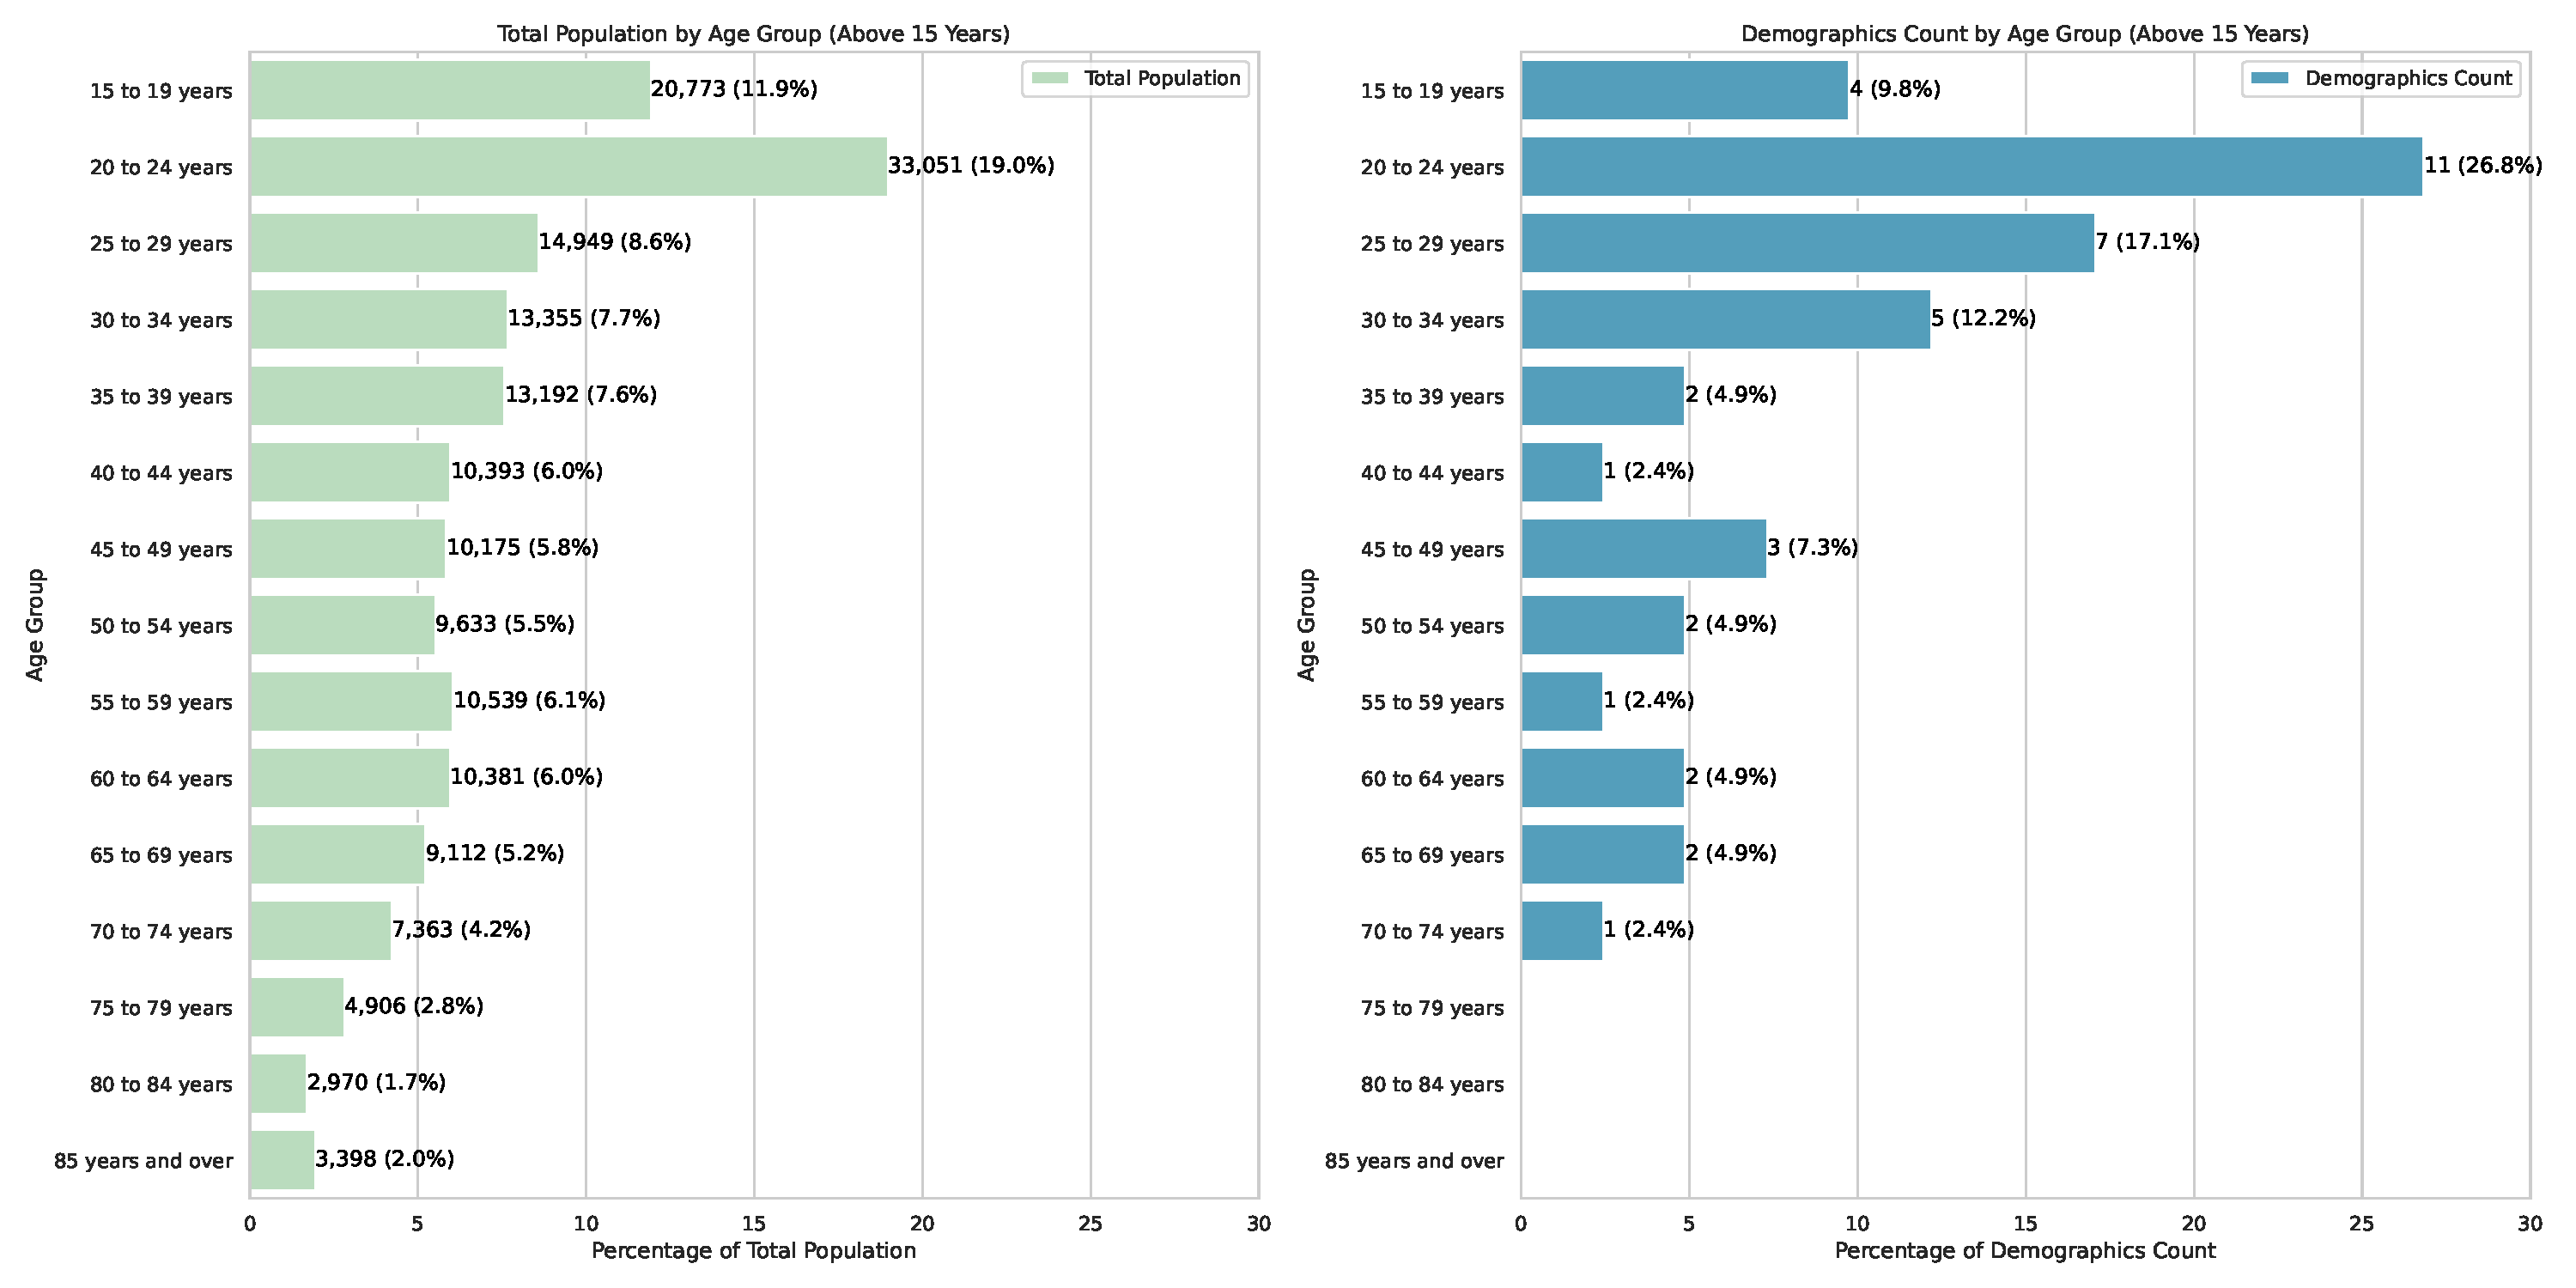
\includegraphics[width=\textwidth]{content/image/demo/demo_age_group.pdf}
        \caption{Age distribution}
        \label{fig:demoAge}
    \end{subfigure}
    \hfill
    \begin{subfigure}[b]{0.3\textwidth}
        \centering
        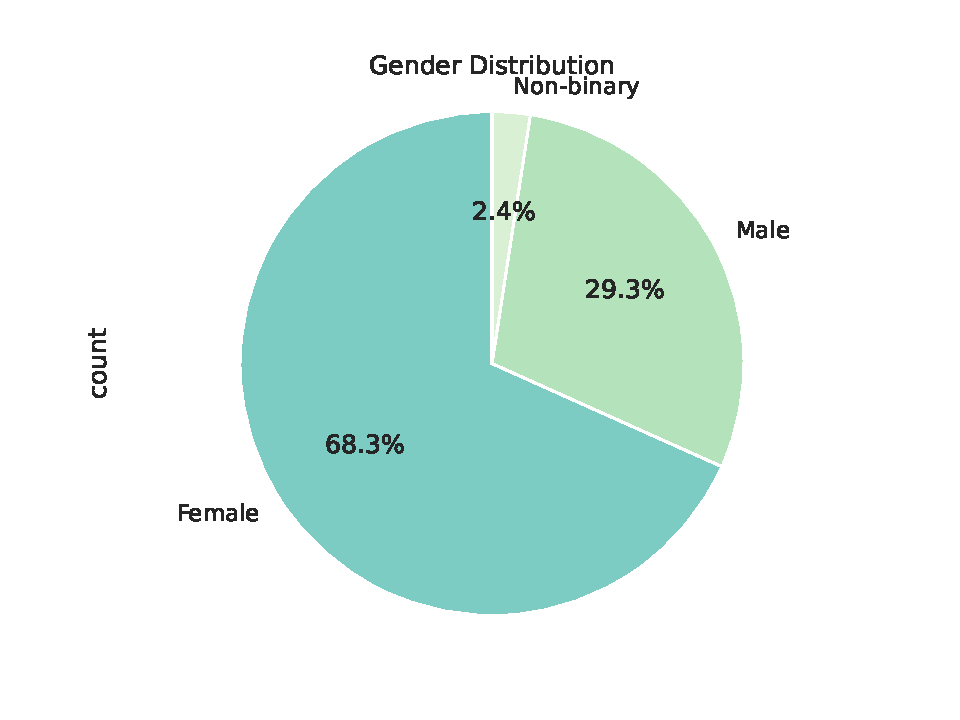
\includegraphics[width=\textwidth]{content/image/demo/demo_gender.pdf}
        \caption{Gender distribution}
        \label{fig:demoGender}
    \end{subfigure}
    \caption{Two figures side by side}
    \label{fig:Demographics}
\end{figure}

% maybe more the figure to the appendix?

\subsection{Demographics}
We recruited a total of $41$ participants, $10$ for each experiment condition. One participant was removed due to data quality concerns. The age of the participants has a mean centered at $34.63$ years old with the full distribution of the participant age distribution to the right of Figure~\ref{fig:demoAge}. The population of the county is presented to the left in the figure. We see that the recruited participants follow closely with the population only missing a few percentages in the $35$-$45$ range making the recruited sample size slightly younger. Recruited participants were more female than male as shown in Figure~\ref{fig:demoGender}.

In terms of ethnicity, $51.2\%$ of the respondents self-identify as White, followed by $26.8\%$ as Asian, $4.9\%$ as Hispanic, and $7.3\%$ as African American. Additionally, $9.8\%$ of participants identify as having mixed ethnicity.

\subsection{Cognitive Load Results}

\begin{figure}[h]
    \centering
    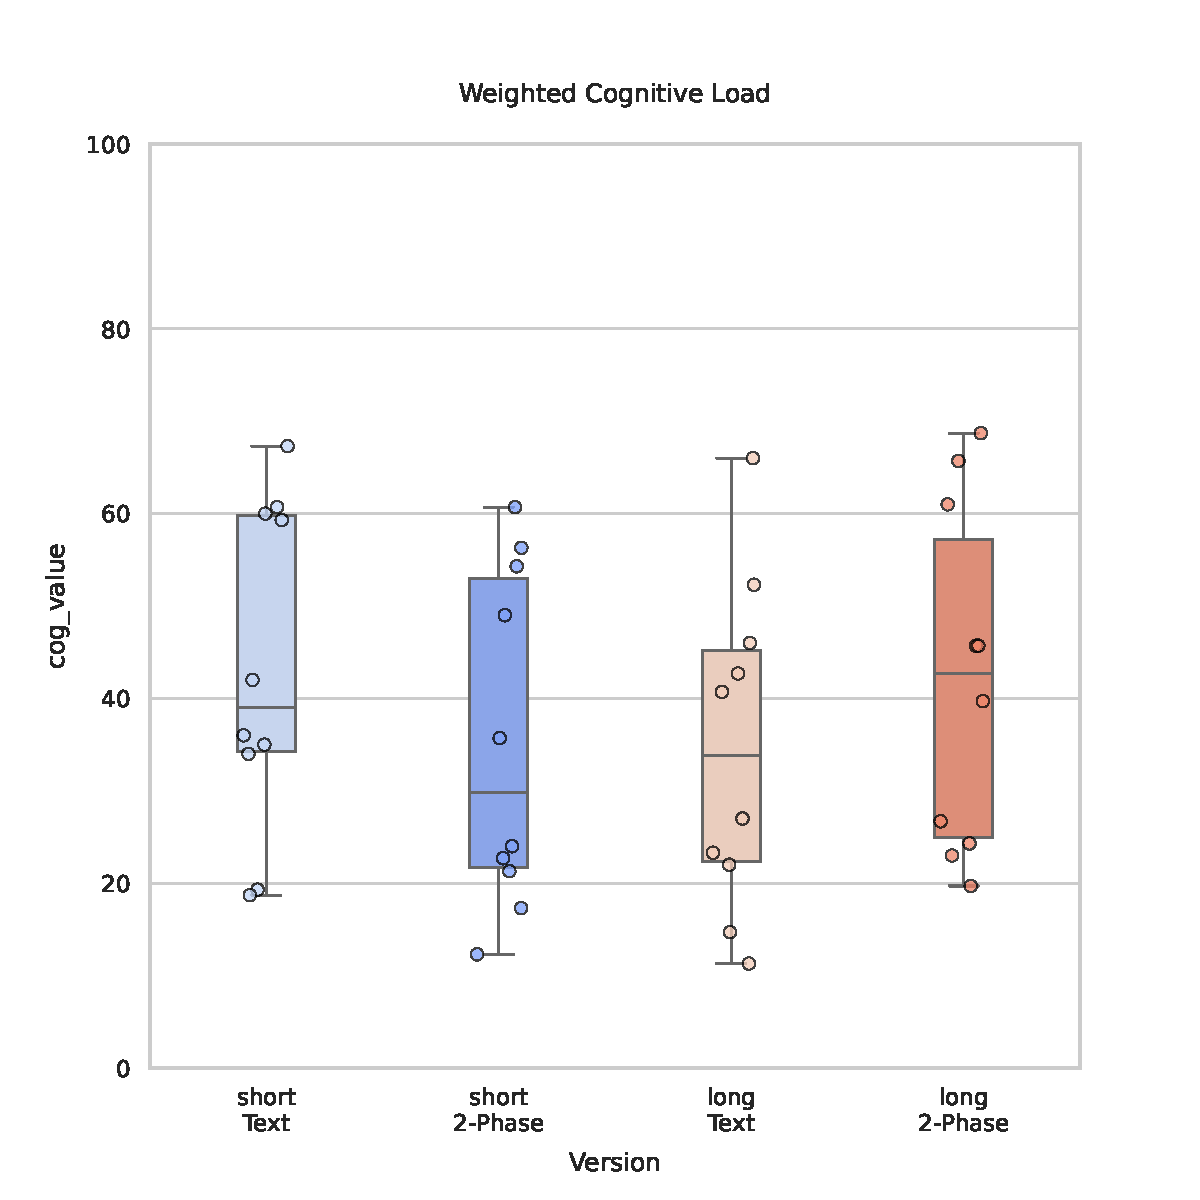
\includegraphics[width=0.5\textwidth]{content/image/results/nasatlx_final_value.pdf}
    \caption{NASA-TLX Results}
    \label{fig:nasatlx-final}
\end{figure}

We show the NASA-TLX weighted results in Figure~\ref{fig:nasatlx-final}. Qualitatively, there is a decrease in cognitive load when comparing short surveys between the text-based interface and interactive interfaces. Conversely, there is an increase in cognitive load when comparing the long survey between the text-based interface and interactive interfaces. However, we are not able to demonstrate statistical significance between the four groups using the Mann-Whitney U test. Reviewing the overall cognitive load, QS participants experienced a `Somewhat High' and `High' cognitive load regardless of length and interface~\cite{hart1988development}. (Need to get the exact percentage).

\begin{figure}[h]
    \centering
    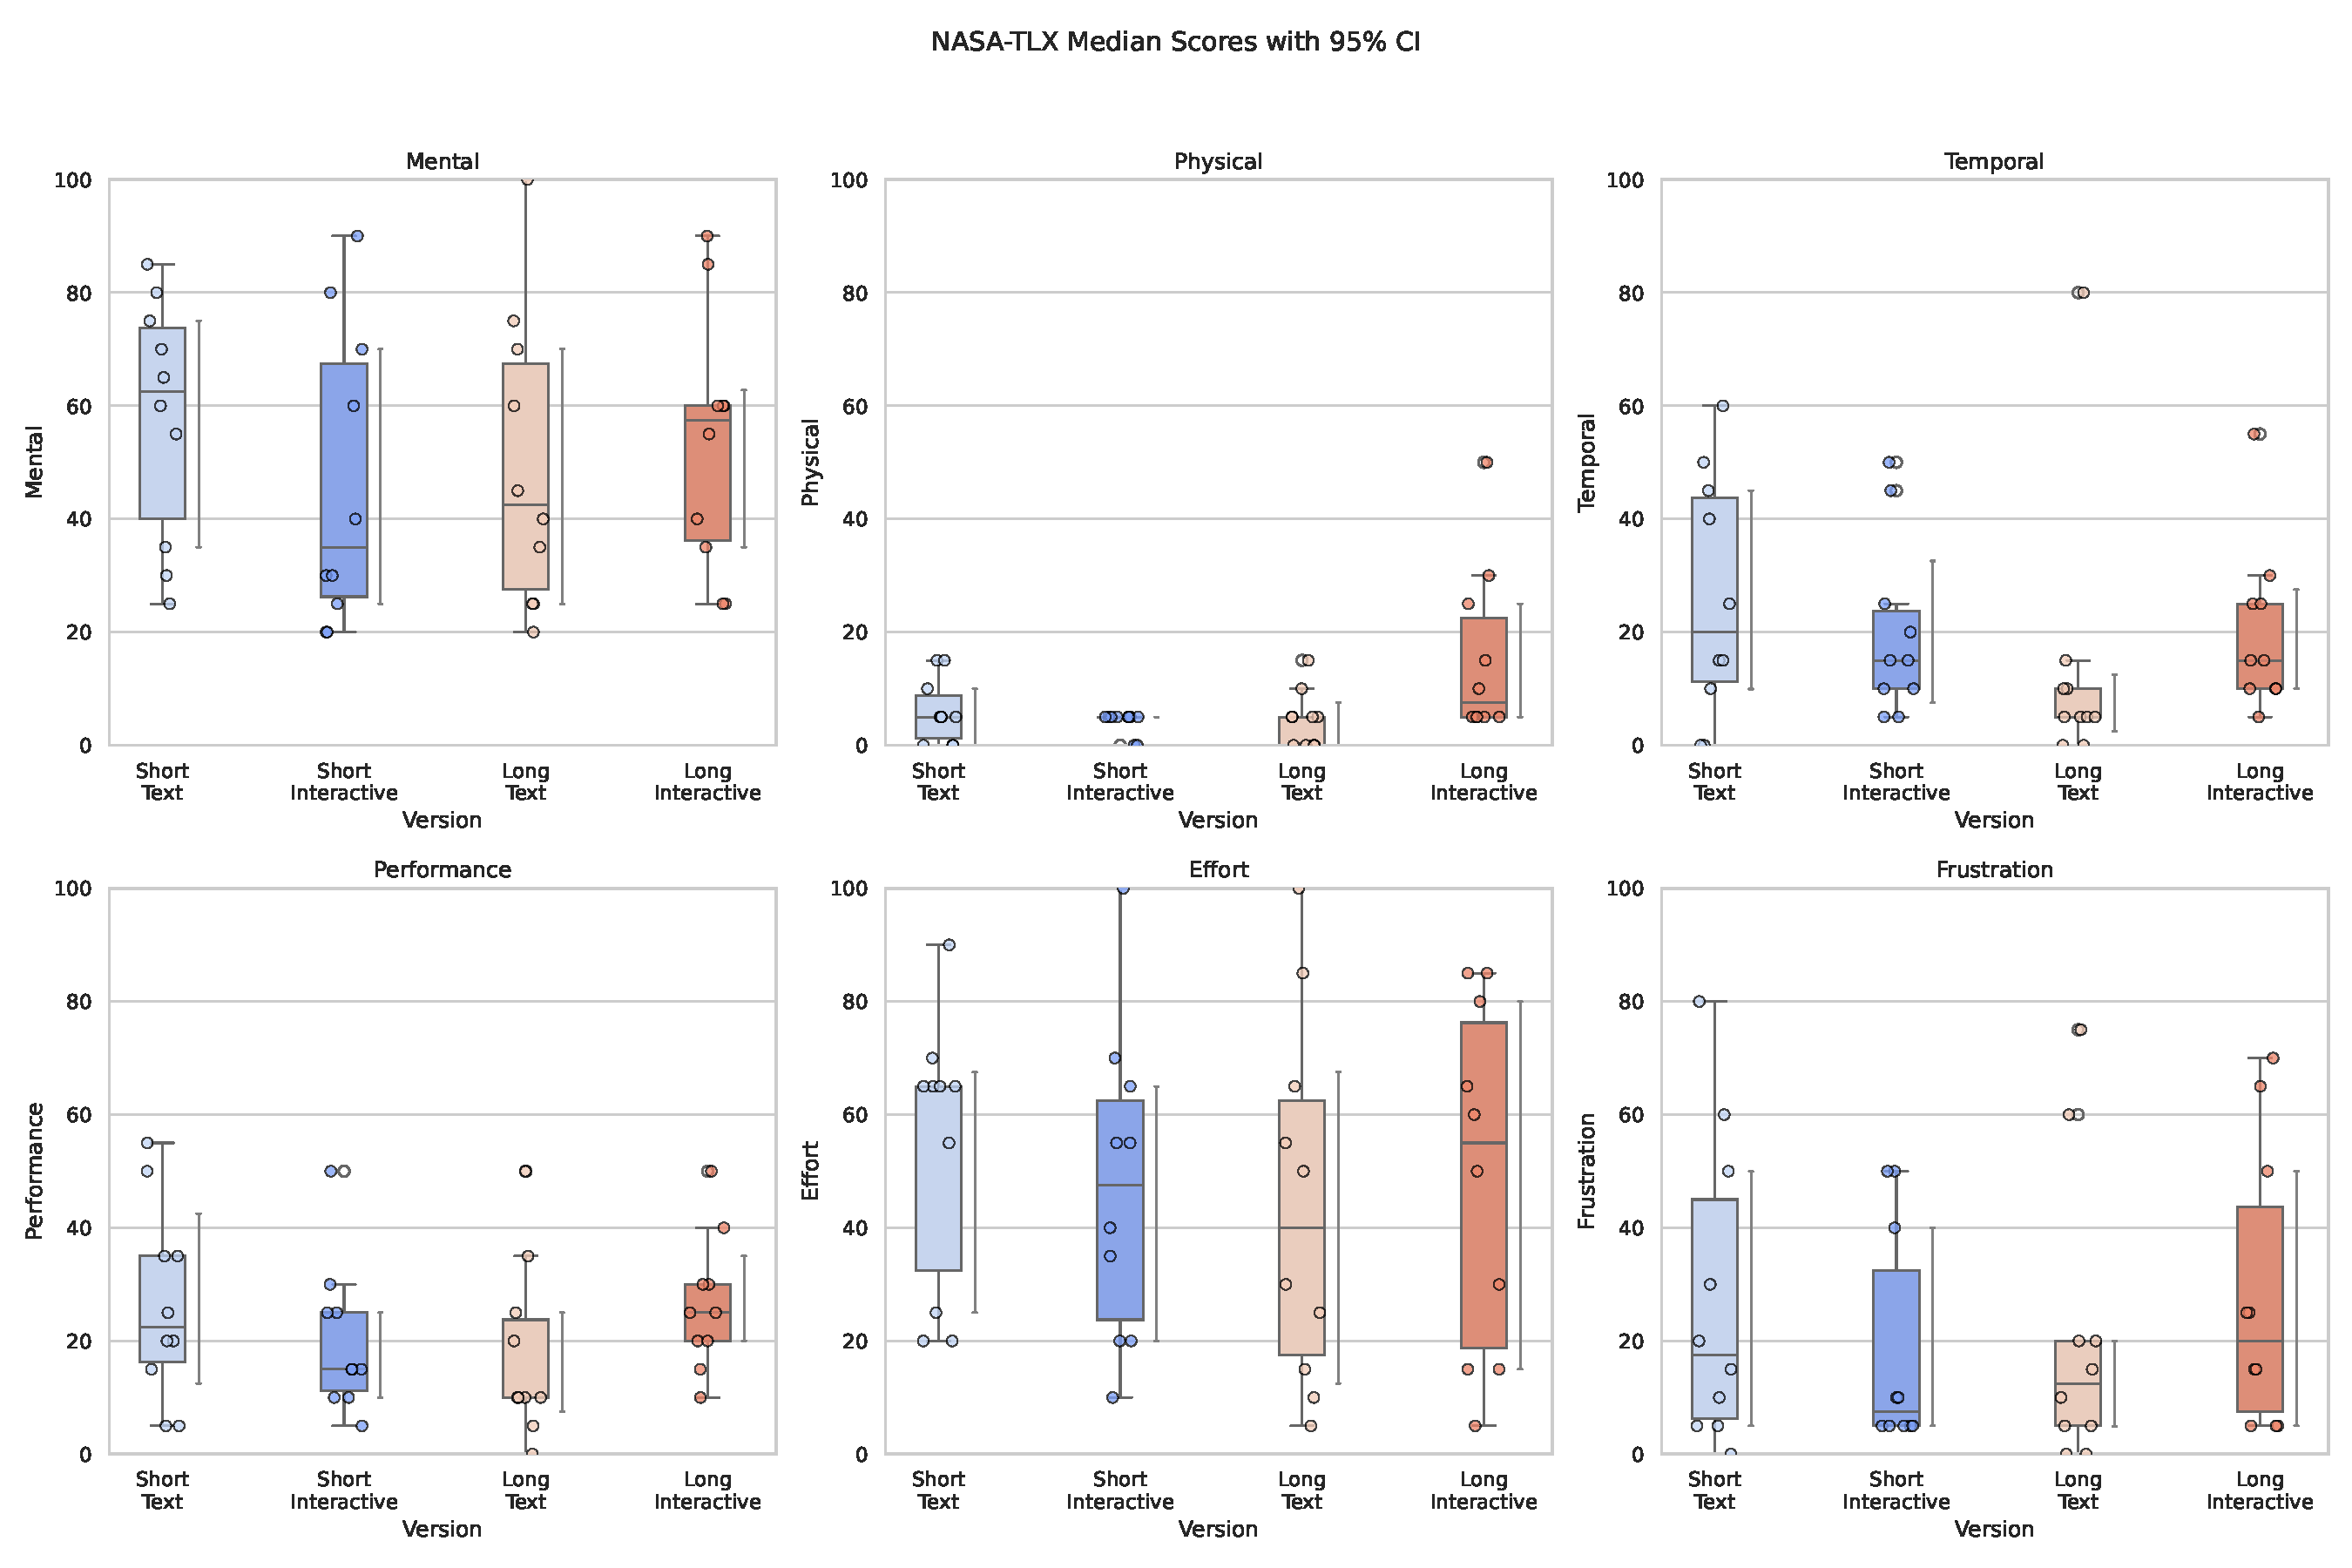
\includegraphics[width=\textwidth]{content/image/results/nasatlx_final_value_with_CI.pdf}
    \caption{NASA-TLX Results}
    \label{fig:nasatlx-with-ci}
\end{figure}

Next, we present the raw scores from the six measurements of NASA-TLX: Mental Demand, Physical Demand, Temporal Demand, Performance, Effort, and Frustration in Figure~\ref{fig:nasatlx-with-ci}. We also show the 95\% confidence interval around the mean for each boxplot.

Mental Demand remains high across all four conditions with a wide variance of responses. The short interactive interface has the lowest median score across all conditions. We see no statistical significance between conditions. For Physical Demand, all conditions except Long Interactive showed minimal scores, with the Long Interactive condition having a noticeably higher median score. There is statistical significance between short and long interactive interfaces ($p<0.01$) as well as text and interactive interfaces in long surveys ($p<0.05$).

Temporal Demand showed more variation across groups. It is interesting to see that the median across the short text interface is among the highest compared to the rest of the groups, while the long-text interface showed the least Temporal Demand. Our statistical tests showed a significant difference between the long text interface and the long interactive interface ($p<0.05$). Performance scores are relatively low across all conditions, indicating that participants experienced less cognitive load from performance. Effort scores echo the mental demand, showing a wide distribution with a high median across the four groups. Lastly, regarding Frustration, we observe qualitatively that the short text interface has a higher median value than the short interactive interface. The opposite is observed in longer surveys, where respondents in the long survey with a text interface experienced less frustration than the interactive version based on median values. We cannot establish statistical significance in the latter three aspects of NASA-TLX.

Based on these results, given the small sample size for each group of participants, we were not surprised that most results do not provide statistical significance in changes in cognitive load values. However, there are some trends that we capture via descriptive statistics. First, comparing the overall cognitive load and the breakdown of the sub-components between text interface and interactive interface across the short survey, we see a general trend in a reduction of cognitive load. Next, we are surprised by the upward trend between the text and interactive interface for the longer list. This is against our original hypothesis that under even complex situations, we should see a clearer portrait of how interactive interactions can reduce cognitive load. While it is possible that interactive interfaces can increase study participants' cognitive load, our qualitative results do not hint at this possibility. In addition, comparing the long and short survey in the text-based interface, it is counter intuitive to see a downward trend across cognitive load. Logically, choosing among more options would demonstrate a higher cognitive load.

These results lead us to further investigate the source of cognitive demands and participants' behaviors.

\subsubsection{Mental Demand}
Participants highlighted various sources that contributed towards their mental demand. In this section, we first highlight similarly across the groups, then we highlight the differences. The two main sources of mental demand is expected. Participants exacerbated higher mental demand due to two major source:~\textit{Budget management} and~\textit{Preference construction}.

\paragraph{Budget management} Participants aimed to consume the given credit to complete QS. $17$ participants experienced increase in mental demand due to budgeting within the limited credit (N=4), tracking remaining credit (N=10), and trying to maximize spend (N=8). When asked about where participants experienced mental demand:

\begin{displayquote}
How many I got left that~\ldots\ that I haven't voted on yet, and seeing if I and looking at the remaining credits, I'm trying to mentally divide that up before I start allocating upvotes and downvotes.

\small{\noindent \hfill -- S006, long interactive interface}
\end{displayquote}


\begin{displayquote}
And then I just wanted to make sure that I used all the credit that I had available to me, and also knowing that in order to like show your support for certain societal issues you had to like that was giving a tangential take away from other societal issues that you could support as well.
    
\noindent \hfill -- S032, short text interface.
\end{displayquote}

\paragraph{Preference construction} Participants (N=36) experience increase in mental demand due to preference construction. We can break it down into determining relative preference (N=16) where participants focuses on internal evaluation and comparison among different options; option prioritization (N=17) where participants need to make trade-offs to elicit high priority options and translate internal preferences to a subselection of options; and precice resource allocation (N=30) where a value or adjustment need to represent their preferences.

\begin{displayquote}
Figuring out my priorities, and how much I prioritize option 1 over option 2. What is the difference between those 2 on my priority list?

\hfill -- S002, short interactive interface, determining relative preference
\end{displayquote}

% I think the whole time I was trying to balance, I think II think I partly was discovering my what's the word I want to use bias isn't quite right. My priorities (S031, I)

\begin{displayquote}
I knew which ones that I wanted to dedicate the most to, and I knew which one I wanted to dedicate the least to. But it was that middle area that was kind of a grey area.
    
\noindent \hfill -- S008, short interactive interface, option prioritization
\end{displayquote}

% I knew which ones that I wanted to dedicate the most to, and I knew which one I wanted to dedicate the least to. But it was that middle area that was kind of a grey area.
% \noindent \hfill -- S024, short text interface, option prioritization

\begin{displayquote}
I'm not sure how to put into words~\ldots like having to pick how many upvotes would go to each one
    
\noindent \hfill -- S023, long text interface, precice resource allocation
\end{displayquote}
% so the interest in mental difficulty was determining how much of my credits I would distribute among the top 3. (S014, III)
% my relative preference like, should 6 support good enough? Or should I give several upvotes (S007, III)

While preference construction is the main source of mental demand across all experiment groups, we noticed a distinct difference in the scope, especially when we compare long text and interactive interfaces. Participants using a long text interface experience higher mental demand on preference construction and preference, where they tend to \textit{think about issues more narrowly, focusing on personal relevance}. If we consider all nine participants experiencing mental demand from preference construction, $8$ of them experessed a narrower view and only $4$ discussed about hollistic consideration.

\begin{displayquote}
\bracketellipsis also seeing the long list and obviously having to pick between quite a few things that I do feel very strongly about and having to figure out which ones do, I feel more strongly about than others.
    
\noindent \hfill -- S023, long text interface
\end{displayquote}

\begin{displayquote}
Trying to figure out what upvotes I should give it you know~\ldots compared to~\ldots I even kind of went back compared to the other topics: education compared to medical research, and even with like adult education, I kind of went back and forth between those two. \bracketellipsis So it was very mental tasking for me.

\noindent \hfill -- S015, long text interface
\end{displayquote}
In both quotes, both participants are making tradeoffs within a narrow focus or decising a specific value among a handful of options. In contrast, participants using a long interactive interface's high mental demand on preference construction and preference is primarily sourced from \textit{considering the broader societal impact and evaluating options more holistically}. Among all 10 participants, $9$ of them expressed a hollistic view compared to only $3$ expressed a narrower view.

\begin{displayquote}
\bracketellipsis really having to think, especially with so many different societal issues. How do I personally prioritize them? And to what extent do I prioritize them?
    
\noindent \hfill -- S009, long interactive interface
\end{displayquote}

\begin{displayquote}
\bracketellipsis really going through the rest of the categories and deciding okay, which are the pressing issues of our time and which are the pressing issues for this particular society that that I live in. \bracketellipsis You know these causes need a lot more funding, and and others can probably still have some sort of an impact, even with less resources.

\noindent \hfill -- S019, long interactive interface
\end{displayquote}

While this is subtle, the exposure to all the options through the organization phase seems to force participants to think through these options created such responses. This further translated to the operational aspect of the two groups mental demand. Participants that mentioned a narrower view will describe more demand from developing operational strategies in credit allocation, for example:

\begin{displayquote}
So I wanted to be fair.~\bracketellipsis I actually took my calculator out and said~\bracketellipsis  how much would it be if I equally distributed it and then how do I do that? Do I wanna do it all equally or not?

\noindent \hfill -- S020, long text interface
\end{displayquote}

On the other hand, the hollistic view lead to mental demand coming from statigic planning and forming processes to operate upon. This ability might also came from the interactive interface to support a more complex decision making process.

\begin{displayquote}
I wanted to make sure I wanted to give some credit to everything~\bracketellipsis I'm trying to make sure that I had without doing a lot of~\ldots I guess redos is trying to kind of get it right the first time on how I weight things.

\noindent \hfill -- S032, long interactive interface
\end{displayquote}

% IN_T4: Wanting more information on the options (N=6/40)
% 5. While the numbers seem small, non of this request came from v3. This could explain that participants are already overloaded from the existing the task.

\subsubsection{Physical Demand}
Regarding physical demand, most participants reported minimal or no physical demand. Participants primarily attributed physical demand to reading text on the screen ($N=4$), using the mouse ($N=16$), or moving their head to navigate the vertical screen ($N=5$). However, they emphasized that these demands were minimal. Notably, slightly more participants in the interactive interface group ($N=11$) mentioned physical demand from using the mouse, reflecting their increased interaction with the interface.

\subsubsection{Temporal Demand}
We derived four major sources of causes for temporal demand across groups:~\textit{Decision Complexity},~\textit{Budget management},~\textit{Operational Efficicenty}, and~\textit{Strategic Decision Making}.

\paragraph{Decision Complexity}
Decision complexity involves participants experiencing temporal demand because there are many decisions to make (i.e., deciding votes for each option) or them feeling concerned about the time and effort already invested (i.e., their sunk cost) representing the complexity of the tasks. While each experiment group all has participants expressing sources of temporal demand from either types, participants in the long interactive interface group (N=4) express their challenge with making multiple decisions. $1$ participant from the rest of the other three groups expressed similiar experiences. It is reasonable since short surveys has much less options to consider. Also, this reflects our observation in the other demands , where this group of participants constantly considers options holistically. We see participants mention about the time spent on pairwise comparisons:
\begin{displayquote}
~\bracketellipsis but when you are being presenting the ideas that they're that they are being put together, and you need to allocate the resources. Say, you know, this one is more important than that one. That's the part when it gets tricky, so that you spend more time here.
    
\noindent \hfill -- S037, long interactive interface
\end{displayquote}

What is more surprising to find is that almost half of the participants (N=4) in the short text interface influenced more by the concerned about the time and effort already invested. The other group had at most $2$ participants express such concern. Participants would mention:

\begin{displayquote}
I didn't see any time anywhere. So at first, so at first it was like, Okay, this is fine. But then on the end, I was like, maybe I should just hurry up and make a decision. So it's like at first it would been here, but then I kinda moved up near the end when I was hanging a waffling between my upvotes.
        
\noindent \hfill -- S024, short text interface
\end{displayquote}

We try to explain this after also examing the operational efficiency.

\paragraph{Operational Efficicenty}
Next, we turn to Operational Efficiency, which represents the sources where participants describe them wanting to finish the survey, execute operations (i.e., reading), or making a decision via a specific operation (i.e., update vote values) efficicenty. Over half of the short survey participants (5 for text interface and 6 for interactive interface) highlighted this as source of temporal demand verses half from the long (N=5, 3 from text and 2 from interactive interfaces) group. Participants would say:

\begin{displayquote}
I wanna get through things in an efficient manner which doesn't necessarily mean I rush it. But it does mean that I do things expeditiously. Especially. I'd like to think I'm somewhat computer-savvy. And so to be able to move through this quickly and efficiently. I do take pride in, but it's all personal stuff. It's not nothing outwardly influencing me. 
        
\noindent \hfill -- S032, short text interface
\end{displayquote}

\begin{displayquote}
I want the credit done but I don't want to be overthinking.
            
\noindent \hfill -- S013, short text interface
\end{displayquote}

Taking~\textit{Decision Complexity} and~\textit{Operational Efficicenty} altogether, we interperate that the participants in the short survey created a misperception that this is a simple task (seeing just $6$ options on the screen). The participants in the interactive interface was forced to slow down through the organization phase which also assisted in constructing some preferences, preparing them to decide values for the votes.

\paragraph{Budget Management}
A few participants (N=4) mentioned that temporal demand came from budget management. For instance:
\begin{displayquote}
When the money was decreasing, as I was casting more upvotes or downvotes so as the money decreases I felt kind of rushed.
            
\noindent \hfill -- S034, long interactive interface
\end{displayquote}
Participants translated the growing marginal cost of votes into their temporal demand.

\paragraph{Strategic Decision Making}
Five of all participants attributed temporal demand to thinking about strategic approaches in completing the task. 

\begin{displayquote}
I actually went through the whole thing again just to see like, just to compare my votes and see how that was doing so I know that was taking up some lot of time, and I know that there wasn't an expected kind of like participate participation time limit, and I feel like for any of these topics just looking at how kind of important they are.
            
\noindent \hfill -- S001, long text interface
\end{displayquote}

In addition, three participants from the long survey pointed out that the vertical screen and its the ability to see all the options facilitated direct comparisons, and being transparent about the entirety of the task reduced temporal demand. 

\begin{displayquote}
(Seeing) all at once I can see how many there are, so it's kind of like I can kind of tell when I will be done.

\noindent \hfill -- S041, long text interface
\end{displayquote}

\subsubsection{Performance Demand} 
From the quantiative data, participants across four groups express less performance demand compared to aspects such as mental demand and effort. In this section, we again first report sources of this demand shared across groups and then highlight the differences observed. Two principal themes emerged: The first source comes from~\textit{social responsibility} and the latter on~\textit{operational actions}.

\paragraph{Social Responsibility}
Several participants expressed the source of performance demand from accounting~\textit{decision-maker responsibility} (N=8) and from considering~\textit{uncertainity of the outcome} (N=3). Participants would express their guilt that they weren't able to avoid because of specific tradeoffs or that they want to be fair.

\begin{displayquote}
    I don't want people to think that I just like don't care about <ethnicity> people at all. I also don't think like government funding should go towards like religious organizations. You know what I mean. So I don't want somebody to think that like, I just don't care about <ethnicity> people.
    
\noindent \hfill -- S041, long text interface, decision-maker responsibility
\end{displayquote}

In this quote, the participant placeed themselves inside the shoes of a member of the government, rather than a citizen expressing their own attitudes, this shift in project of roles introduced the perforamce demand. This extends further to the participants trying to forsee an outcome:

\begin{displayquote}
If I was actually running a government funding~\bracketellipsis I don't know how this (the survey results) might actually affect people. Some of these things might be unpopular or bad, or have outcomes that I didn't forsee.
    
\noindent \hfill -- S027, short interactive interface, uncertainity of the outcome
\end{displayquote}

\paragraph{Operational Actions}
On the other hand, operational actions involves two specific perspectives. Participants (N=6) highlighted the demand for their performance came from using up all their credits or avoiding overspending their credits. In other words, gaining control in credit management. The other aspect regards assuring that the expressed relative preference is accurate and justified. Participants (N=5) are concerned that they made incorrect interpretation and as reflective of their 'true' preferences. $6$ other participants discussed that they experience performance demand from the bounded time, energy and resources they have in this study, which is an association with the other cognitive demands.

\begin{displayquote}
I don't think I did it perfectly, because I didn't have 0 remaining credits.
    
\noindent \hfill -- S024, short text interface, budget management
\end{displayquote}

\begin{displayquote}
I'm concerned that it's not as reflective of my views as I wanted to be like, or I was concerned about it.~\bracketellipsis I was concerned that maybe it didn't.

\noindent \hfill -- S041, long text interface, preference reflectiveness
\end{displayquote}

While participants experienced performance demand, most participants feel positive about their final submission. However, there are nuance differences across the the degree. We coded participants resposnes into three categories of satisfactory:~\textit{Did their best},~\textit{Feel good}, and~\textit{Good enough}.~\textit{Did their best} refers to when the participants stated that they had exhaused their maximum effort to complete the task.~\textit{Feel good} refers to when the participants expressed positive emotions or satisfaction about their performance or the outcome of their actions.~\textit{Good enough} refers to when the participants acknowledged that their performance or the outcome was acceptable or satisfactory, but not necessarily perfect or the best possible.

Participants that used the interactive interface across short and long groups has almost double the amount of participants (N=11) who expressed~\textit{Feel good} compared to the text interface (N=6). On the other hand, participant using the text interface has more participants (N=5) who expressed~\textit{Did their best} compared to the interactive interface (N=3). This highlighted insights where participants using the interactive interface are more likely to feel good about their performance, while some participants using the text interface are pressed by some challenges.

% TODO: Need to check the reflective thinking part a bit. I **think** there are differences but it is unclear, need to go back to raw code.

\subsubsection{Effort}
Next, we examine the sources of effort that participants experienced. We observed that the source of effort covers the entire operation to complete QS, from constructing preferences, to managing credits, and making tradeoffs. However, in this subsection, we grouped the code into two major categories:~\textit{Operational Effort} and~\textit{Strategic Effort}. We see some differences among the groups regarding these two types of effort.

\paragraph{Operational Effort} This type of effort include individual efforts that focuses on specific behaviors on operating the response within the survey. More specifically, these include navigating the interface, managing the budget at an operational scale (i.e., making sure not to run out of budget, making specific updates between two options), or translating an opinion to a quantifiable adjustment on the survey. We consider these efforts from lower-level operations that directly invole making updates or actions realted to the interface itself. Participants using the text interface (N=14) expressed overwhelminly mentioned sources related to such sources, compared to less than half of the participants from the interactive interface (N=7), with the lowest mention by the long interactive interface group (N=2). We show two examples here where both considered different aspects of operational effort:

\begin{displayquote}
And then I wanted to bump up (an option) maybe to 4 or <option> to 5 and realize I couldn't. My point (number of votes) had to like back down a little bit~\ldots So that would be effort came in of how do I want to really rearrange this to make it (the budget spending) maximize?

\noindent \hfill -- S029, short text interface
\end{displayquote}

\begin{displayquote}
So it was like it was very~\ldots I have to put a lot of effort in terms of you know~\ldots think about each dimension that if I give one credit to <option name> whether it will affect my credits on <another option name>.

\noindent \hfill -- S005, long text interface
\end{displayquote}

\paragraph{Strategic Effort}
We categorize strategic effort into two distinct types:~\textit{personal} and~\textit{global}. Personal strategic efforts involve participants in forming preferences without specifying values and reflecting on their beliefs and values when considering options, thereby translating these strategies into actionable operations. Conversely, global strategic efforts entail participants formulating strategies to align with broader, communal values. This includes ensuring fairness, considering the impact of different options on the entire community, and evaluating the complex relationships between various options.

Notably, nearly twice as many participants (N=7) in the interactive interface expressed effort from global strategic efforts compared to the text interface (N=4). For example,

\begin{displayquote}
Hey, even though I don't really like this idea. But what if they're important? They sort of kind of deserve some attention~\ldots that's why I think I have the effort here.

\noindent \hfill -- S037, long interactive interface
\end{displayquote}

\begin{displayquote}
I think, imagining the trying to imagine every outcome trying to to imagine what what else would be encompassed, encompassed by each category.

\noindent \hfill -- S027, short interactive interface
\end{displayquote}

While the difference in personal strategic efforts was less pronounced, the interactive interface (N=13) was still cited slightly more often as a source of effort than the text interface (N=9). For example,

\begin{displayquote}
It's a lot more involved than just like picking one option, which is why it takes a little more effort.

\noindent \hfill -- S002, short interactive interface
\end{displayquote}
    
\begin{displayquote}
And really the bulk of the effort was how to rank order these (options) and allocate the resources behind the upvotes so that I can accurately depict what I want~\ldots say, a committee to focus on and allocate actual fungible resources, too. 

\noindent \hfill -- S019, long interactive interface
\end{displayquote}

Together, we see that more participants using the interactive interface (N=17) reported sources of strategic effort compared to those using text-based interfaces (N=11). This finding echoes discussions on the sources of mental demand, where participants using the interactive interface tend to think about options holistically. Participants using the text interface have a narrower view when it comes to completing QS.
    

\subsubsection{Frustration}
The source of frustration is categorized into three major themes. These themes are mostly distributed across all experiment groups. These sources can either be~\textit{operational frustration},~\textit{lower level strategic planning}, and~\textit{higher level strategic planning}.

\paragraph{Operational Frustration} Similar to the previous analysis, we define operational frustration as frustration experienced because participants (N=15) wanted to complete an action on the interface. Six participants expressed frustration regarding credit management (i.e., overspending budget); four participants mentioned had trouble deciding the final value for the options; three participants are frustrated because they need to make multiple decisions; five participants were frustrated with the quadratic Mechanism; four participants are frustrated trying to understand the content of the option or how the option connects to them. All experiment groups other than the long text interface (N=2) had almost half of the participants express operational frustration.

\paragraph{lower level strategic planning} This type of frustration relates to frustration that occurs when participants experience conflicts regarding lower-level strategies. Four participants expressed conflict between their personal preferences and what they believe would be other people's preferences. Eight participants experienced conflict between making tradeoffs among a few options. For example:

\begin{displayquote}
Because I know that's important to other people. But it just doesn't to me.
    
\noindent \hfill -- S010, short interactive interface
\end{displayquote}

\begin{displayquote}
I would have loved to have given more to other groups~\ldots and I felt stressed like~\bracketellipsis well~\ldots it's a group that you know is still~\ldots you know~\ldots important~\bracketellipsis
\noindent \hfill -- S020, long text interface
\end{displayquote}

\paragraph{higher level strategic planning} This type of frustration is more fundamental conflicts that participants experienced. For instance, 
\begin{displayquote}
I had to consider how I feel towards that~\ldots how religious media broadcasting is being used in like today's society~\ldots today's political environment. So yeah~\ldots you really have to consider what is important to you. 
\noindent \hfill -- S020, long text interface
\end{displayquote}

participants are facing conflicts that touch on the broader society and their core values of looking at the broader scope. Six other participants expressed something similar. Eight participants felt frustrated because they were forced to make trade-offs among all options instead of a few. For example, 
\begin{displayquote}
I think the frustration is~\ldots I wish that we could help all of these causes, but you know it's just like anything else. You can't do everything and when it's not~\ldots  I feel like it's hard to quantify how much some of these things should be supported versus others. So when you're talking about upvotes and things that's challenging to me, it's frustrating.
\noindent \hfill -- S026, long interactive interface
\end{displayquote}
This result echos the quantitative responses from the NASA-TLX breakdown where long text interface trends slightly lower compared to the other groups. From this analysis, we interpret that frustration comes more from individual's ability to discern and make decisions and not necessarily tied to specific methods in the construction of preference.

\subsection{Interaction Behavior Analysis}
To further investigate the cognitive load results, we focused on participants' behaviors during the survey. Specifically, we aim to understand the time participants spent on the options as well as when a participant makes changes to the survey. When a study participant clicks their mouse on the interface to complete some action, whether it is a drag-and-drop, updating votes, or placing options into a specific group, a timestamp and the payload of the update are stored in the log. The time difference between two actions is attributed to the time the participant took to decide and enact upon a behavior. While participants can be thinking about other things, this is the best proxy we have to study participant behaviors.

\begin{figure}[h]
    \centering
    \begin{subfigure}[b]{0.32\textwidth}
        \centering
        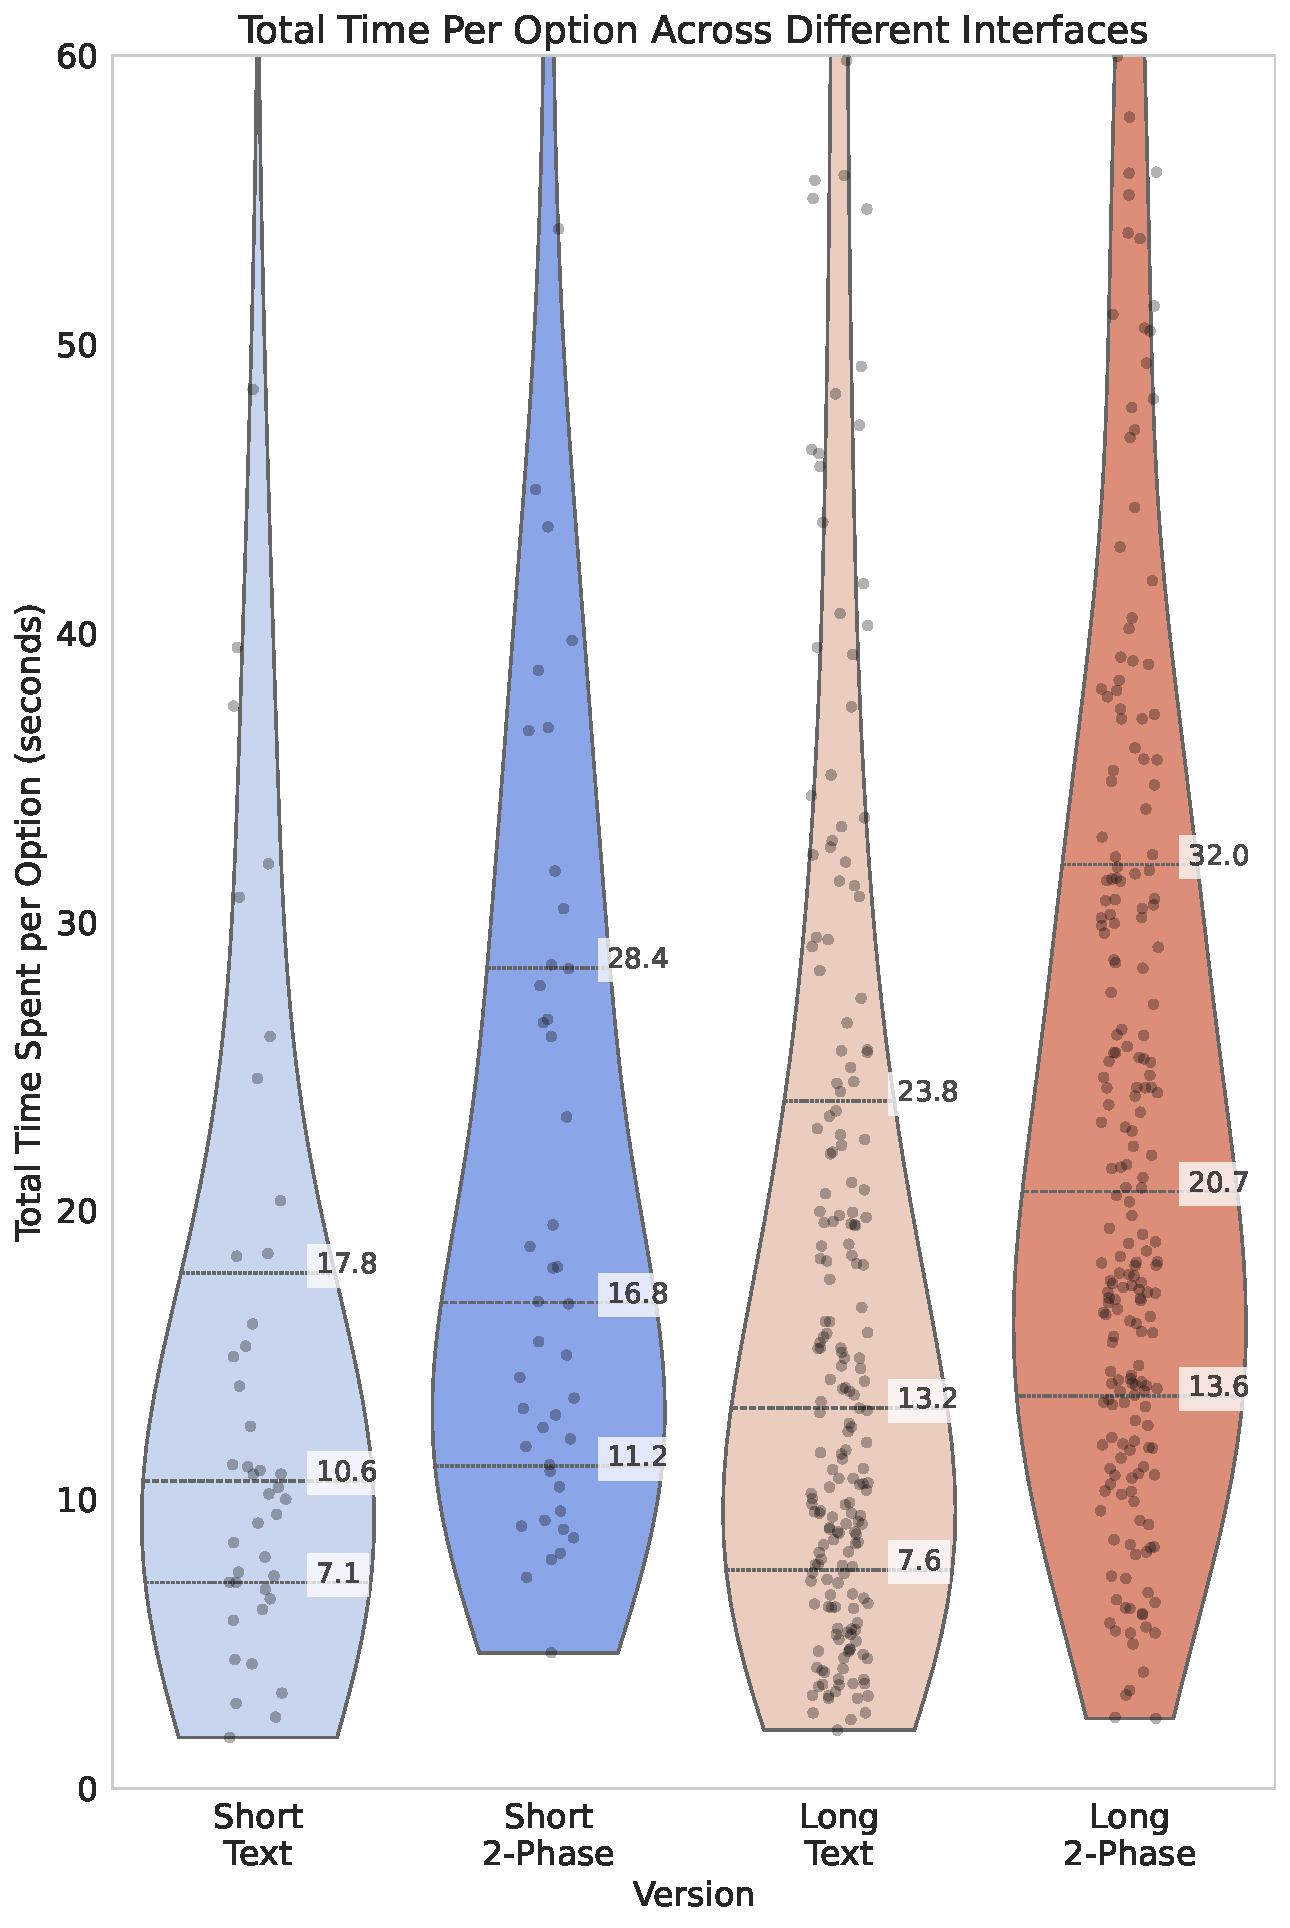
\includegraphics[width=\textwidth]{content/image/results/total_time_per_option.pdf}
        \caption{Total Time per option}
        \label{fig:total_time}
    \end{subfigure}
    \hfill
    \begin{subfigure}[b]{0.32\textwidth}
        \centering
        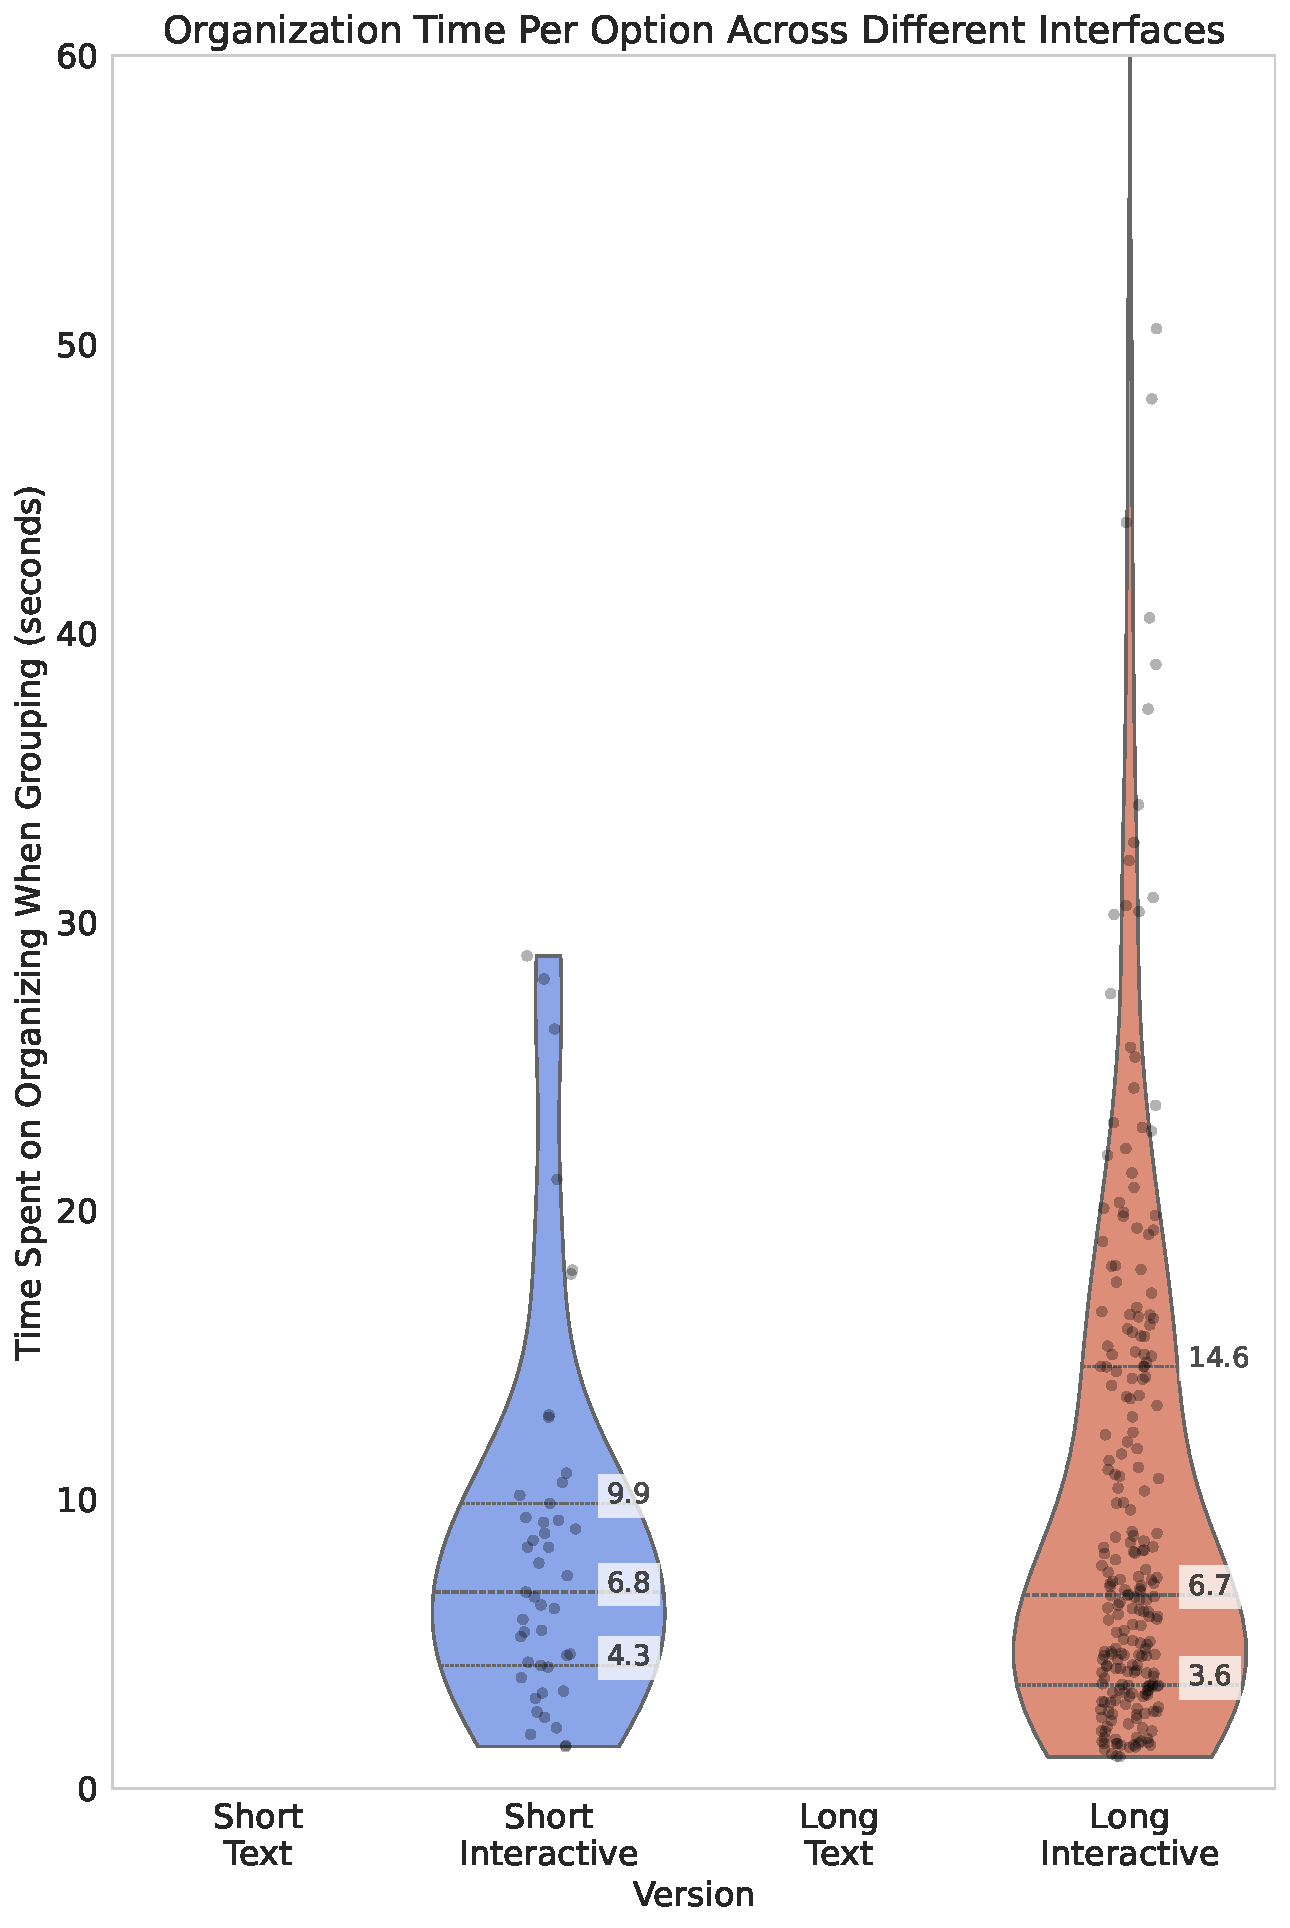
\includegraphics[width=\textwidth]{content/image/results/org_time_per_option.pdf}
        \caption{Organization Time per option}
        \label{fig:org_time}
    \end{subfigure}
    \hfill
    \begin{subfigure}[b]{0.32\textwidth}
        \centering
        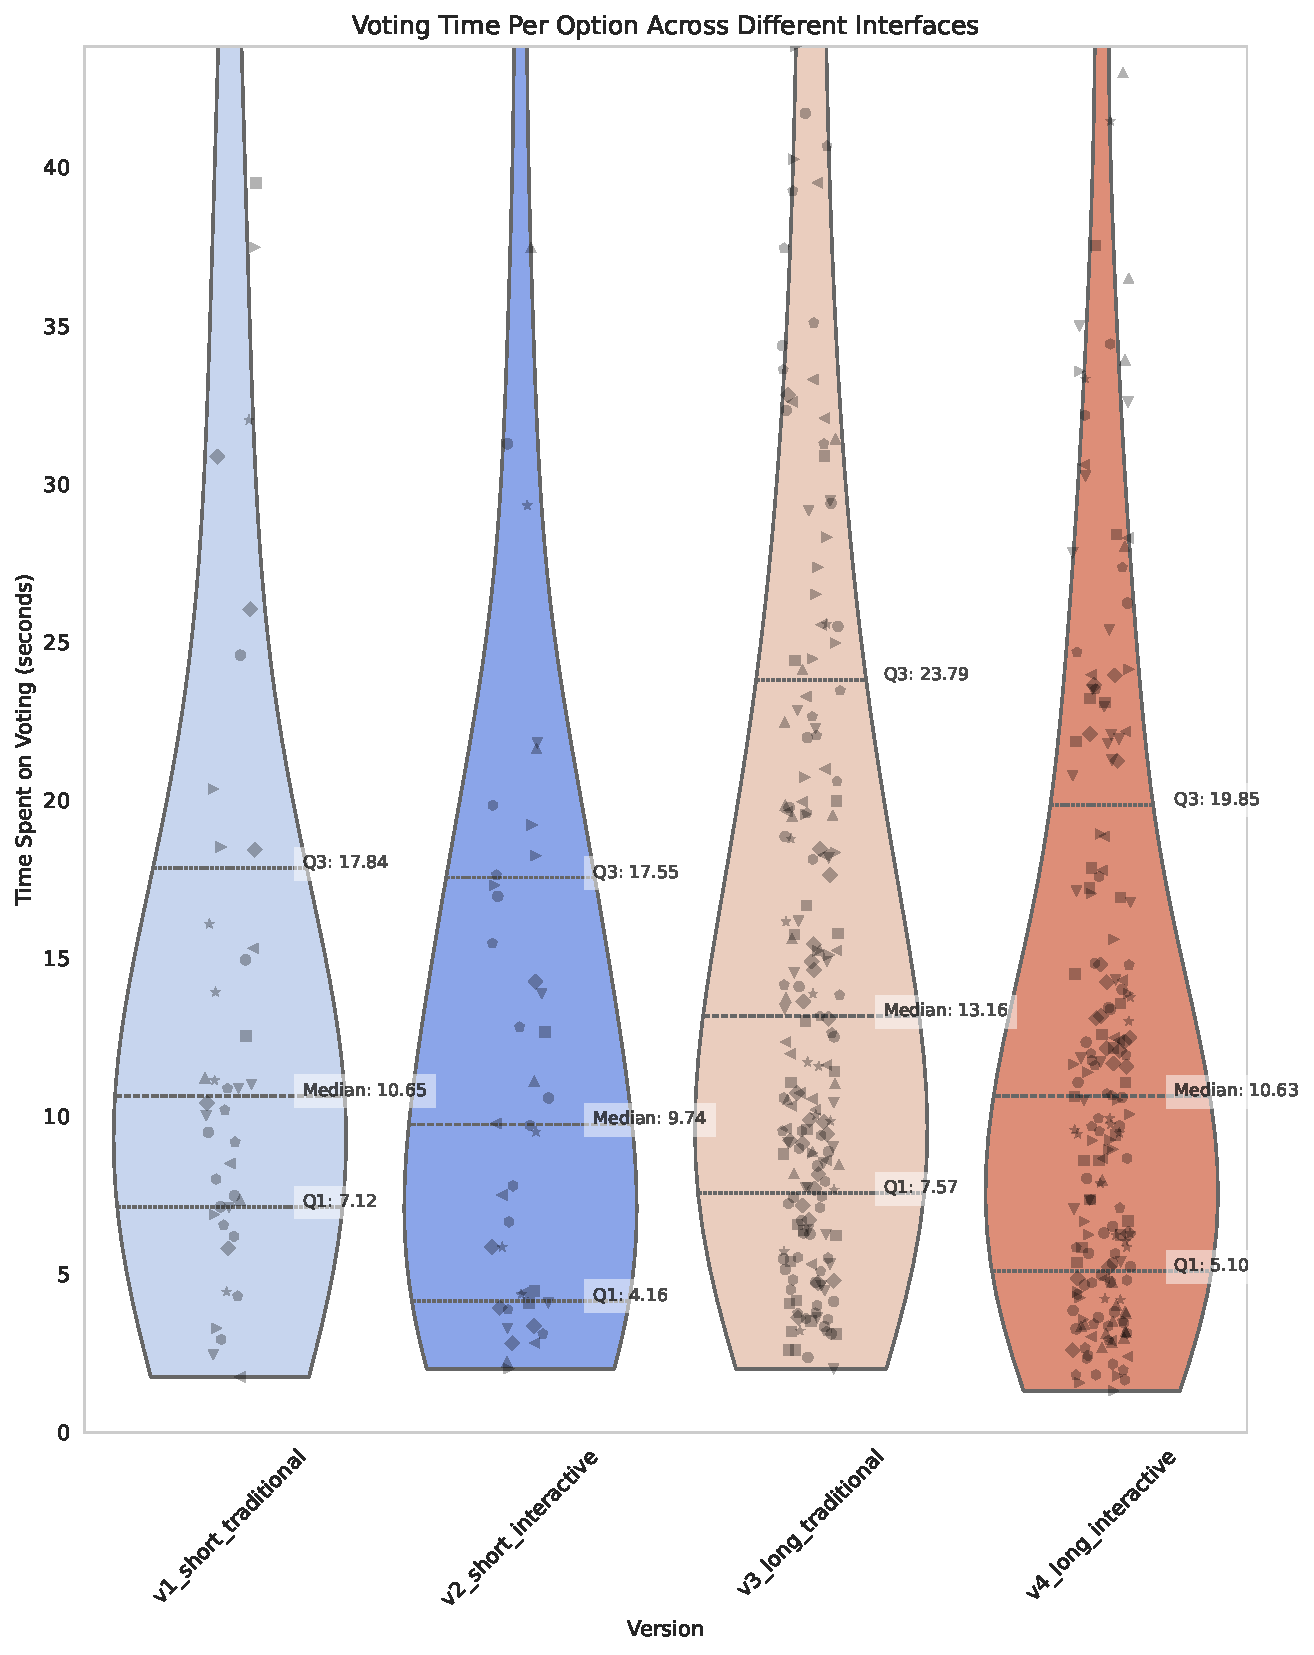
\includegraphics[width=\textwidth]{content/image/results/voting_time_per_option.pdf}
        \caption{Voting Time per option}
        \label{fig:vote_time}
    \end{subfigure}
    \caption{Breakdown of time per option}
    \label{fig:Time Spent Per Option Per Person}
\end{figure}

\subsection{Time Spent per Options}
First, we define time spent per option. A participant can enact several actions related to the same option, for example, a participant might spend $t_1$ time to place the option into a `lean positive' category; spend $t_2$ and $t_3$ time to drag and drop the options to reposition it on the interactive interface; spend $t_4$ and $t_5$ time to update the upvotes on that option. In this case, we would define voting time as $t_4 + t_5$ for that option, and organization time as $t_1 + t_2 + t_3$.

To reduce noise, we intentionally drop all the time participants spent on the first option in the organization phase or voting phase. The goal is to reduce the inclusion of time they spent on reading the prompt, forming their preference, or understanding the interface. We present the results in Figure~\ref{fig:Time Spent Per Option Per Person} where each of the dots represents the time accumulated for an option that a participant interacted with. The violin plot shows the distribution of the dots and the three horizontal lines represent the median, 25th percentile, and 75th percentile of the time spent for that interface.

In Figure~\ref{fig:total_time}, we observe that participants spent more time on the interactive interface than the text interface in both short and long surveys. A non-parametric statistical test supports such observation with $p<0.01$ for short and $p<0.0001$ for long surveys. This is not surprising because participants need to review the options and organize them in the interactive interface which takes more time. We break down the total time spent into organization time and voting time in Figure~\ref{fig:org_time} and Figure~\ref{fig:vote_time}.

Once we separate the organization time (Figure~\ref{fig:org_time}) and identify the voting time (Figure~\ref{fig:vote_time}), while there are no statistically significant differences between the text interface and the interactive interface in the short survey, we see a statistically significant reduction ($p<0.01$) in voting time between the text interface and the interactive interface. In other words, our original hypothesis holds in which the two-step design process did facilitate participants in making their decisions.

\begin{figure}[h]
    \centering
    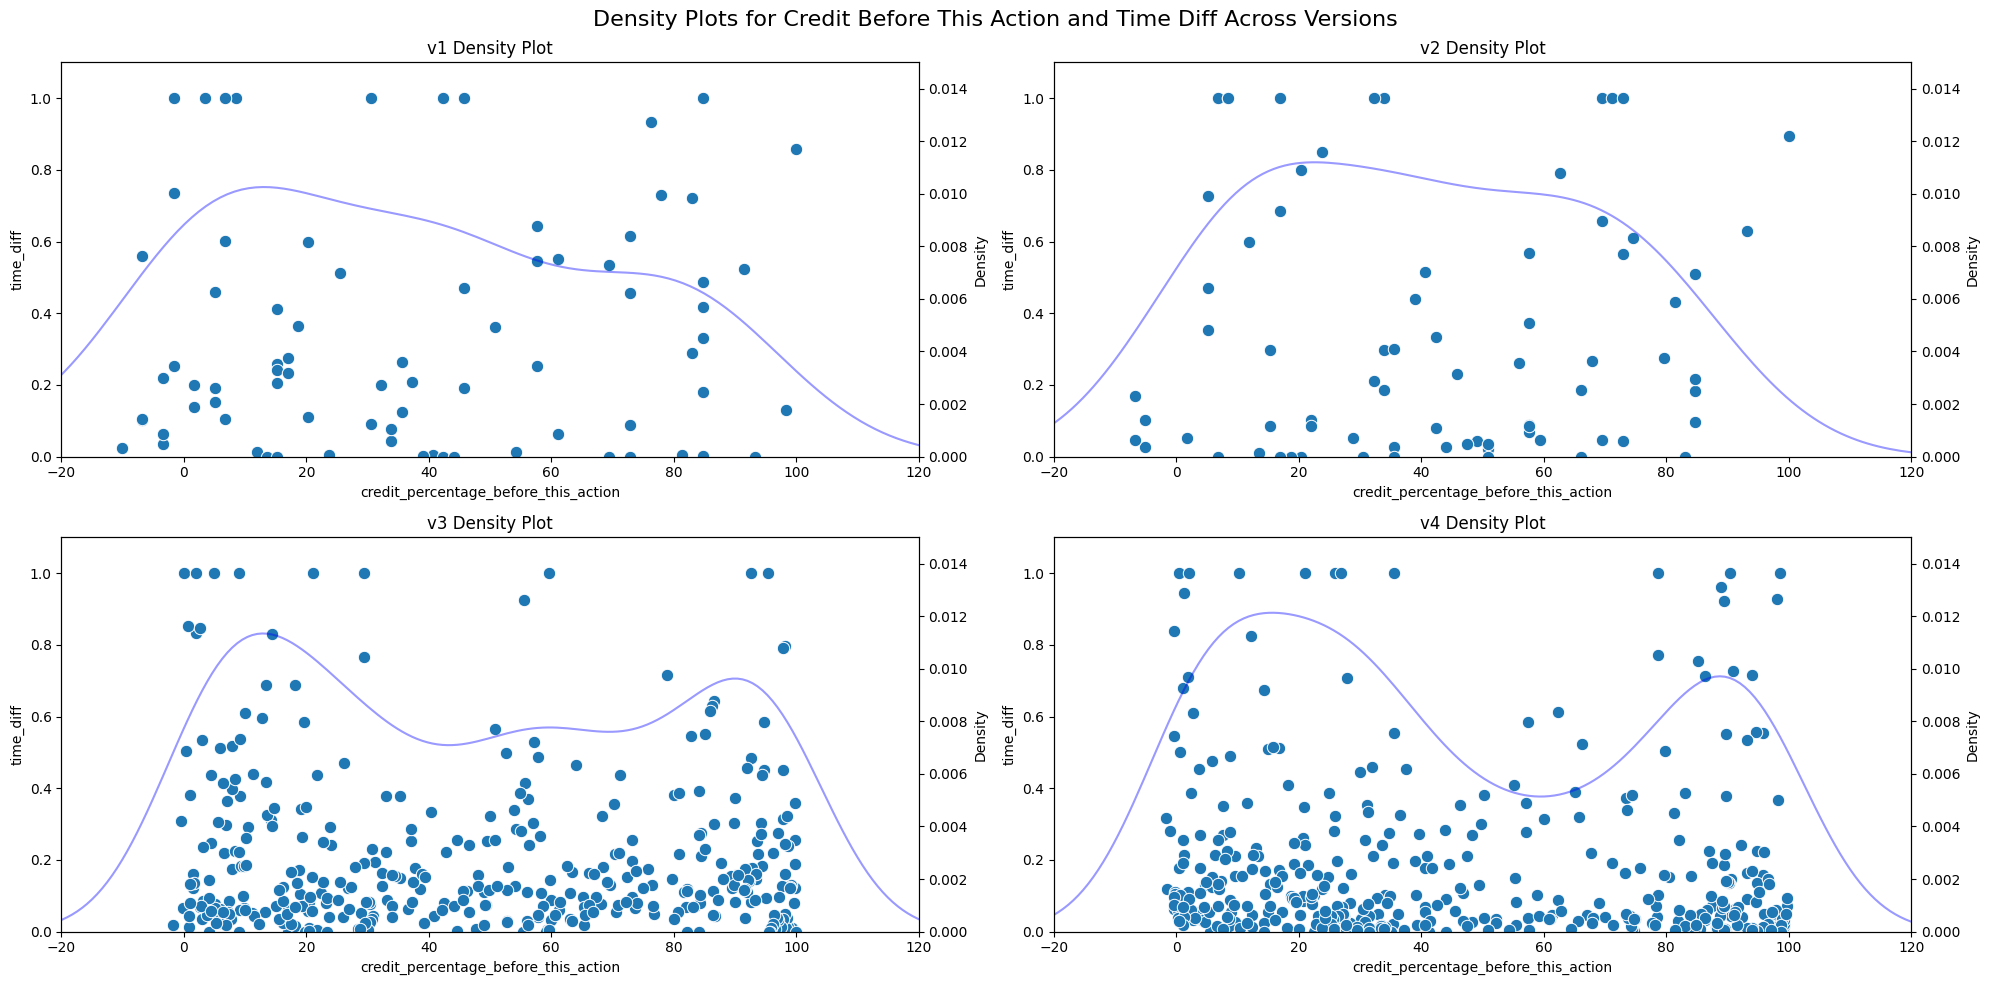
\includegraphics[width=\textwidth]{content/image/results/diff_con.png}
    \caption{voting actions across all options (needs to update chart text, remove normalization, and change the dot colors.)}
    \label{fig:voting_all}
\end{figure}

\subsection{Budget and Voting Behaviors}
Next, we examine participants' voting behavior and how it changed throughout the progress. Given that we observe significant differences in voting time changes comparing text interface and interactive interface for the long option survey, we focus on deciphering the voting action changes between these two experiment conditions in this subsection.

Figure~\ref{fig:voting_all} plots the time of voting actions over the remainder of the participant's budget across the text and interactive interface across all four groups. In other words, different from~\textcite{quarfoot2017quadratic} focusing on the number of accumulated votes over an individual's time, where they showed QV voters make more revisions than Likert Surveys, we focused on the budget scarcity which can influence QS respondents' behaviors.

In this plot, we see two distinct patterns between the short survey and the long survey in terms of participant behaviors. Only in the long surveys did participants exhibit more actions when the budget was abundant and when it began to run out, with the long interactive interface being more significant.

\begin{figure}[h]
    \centering
    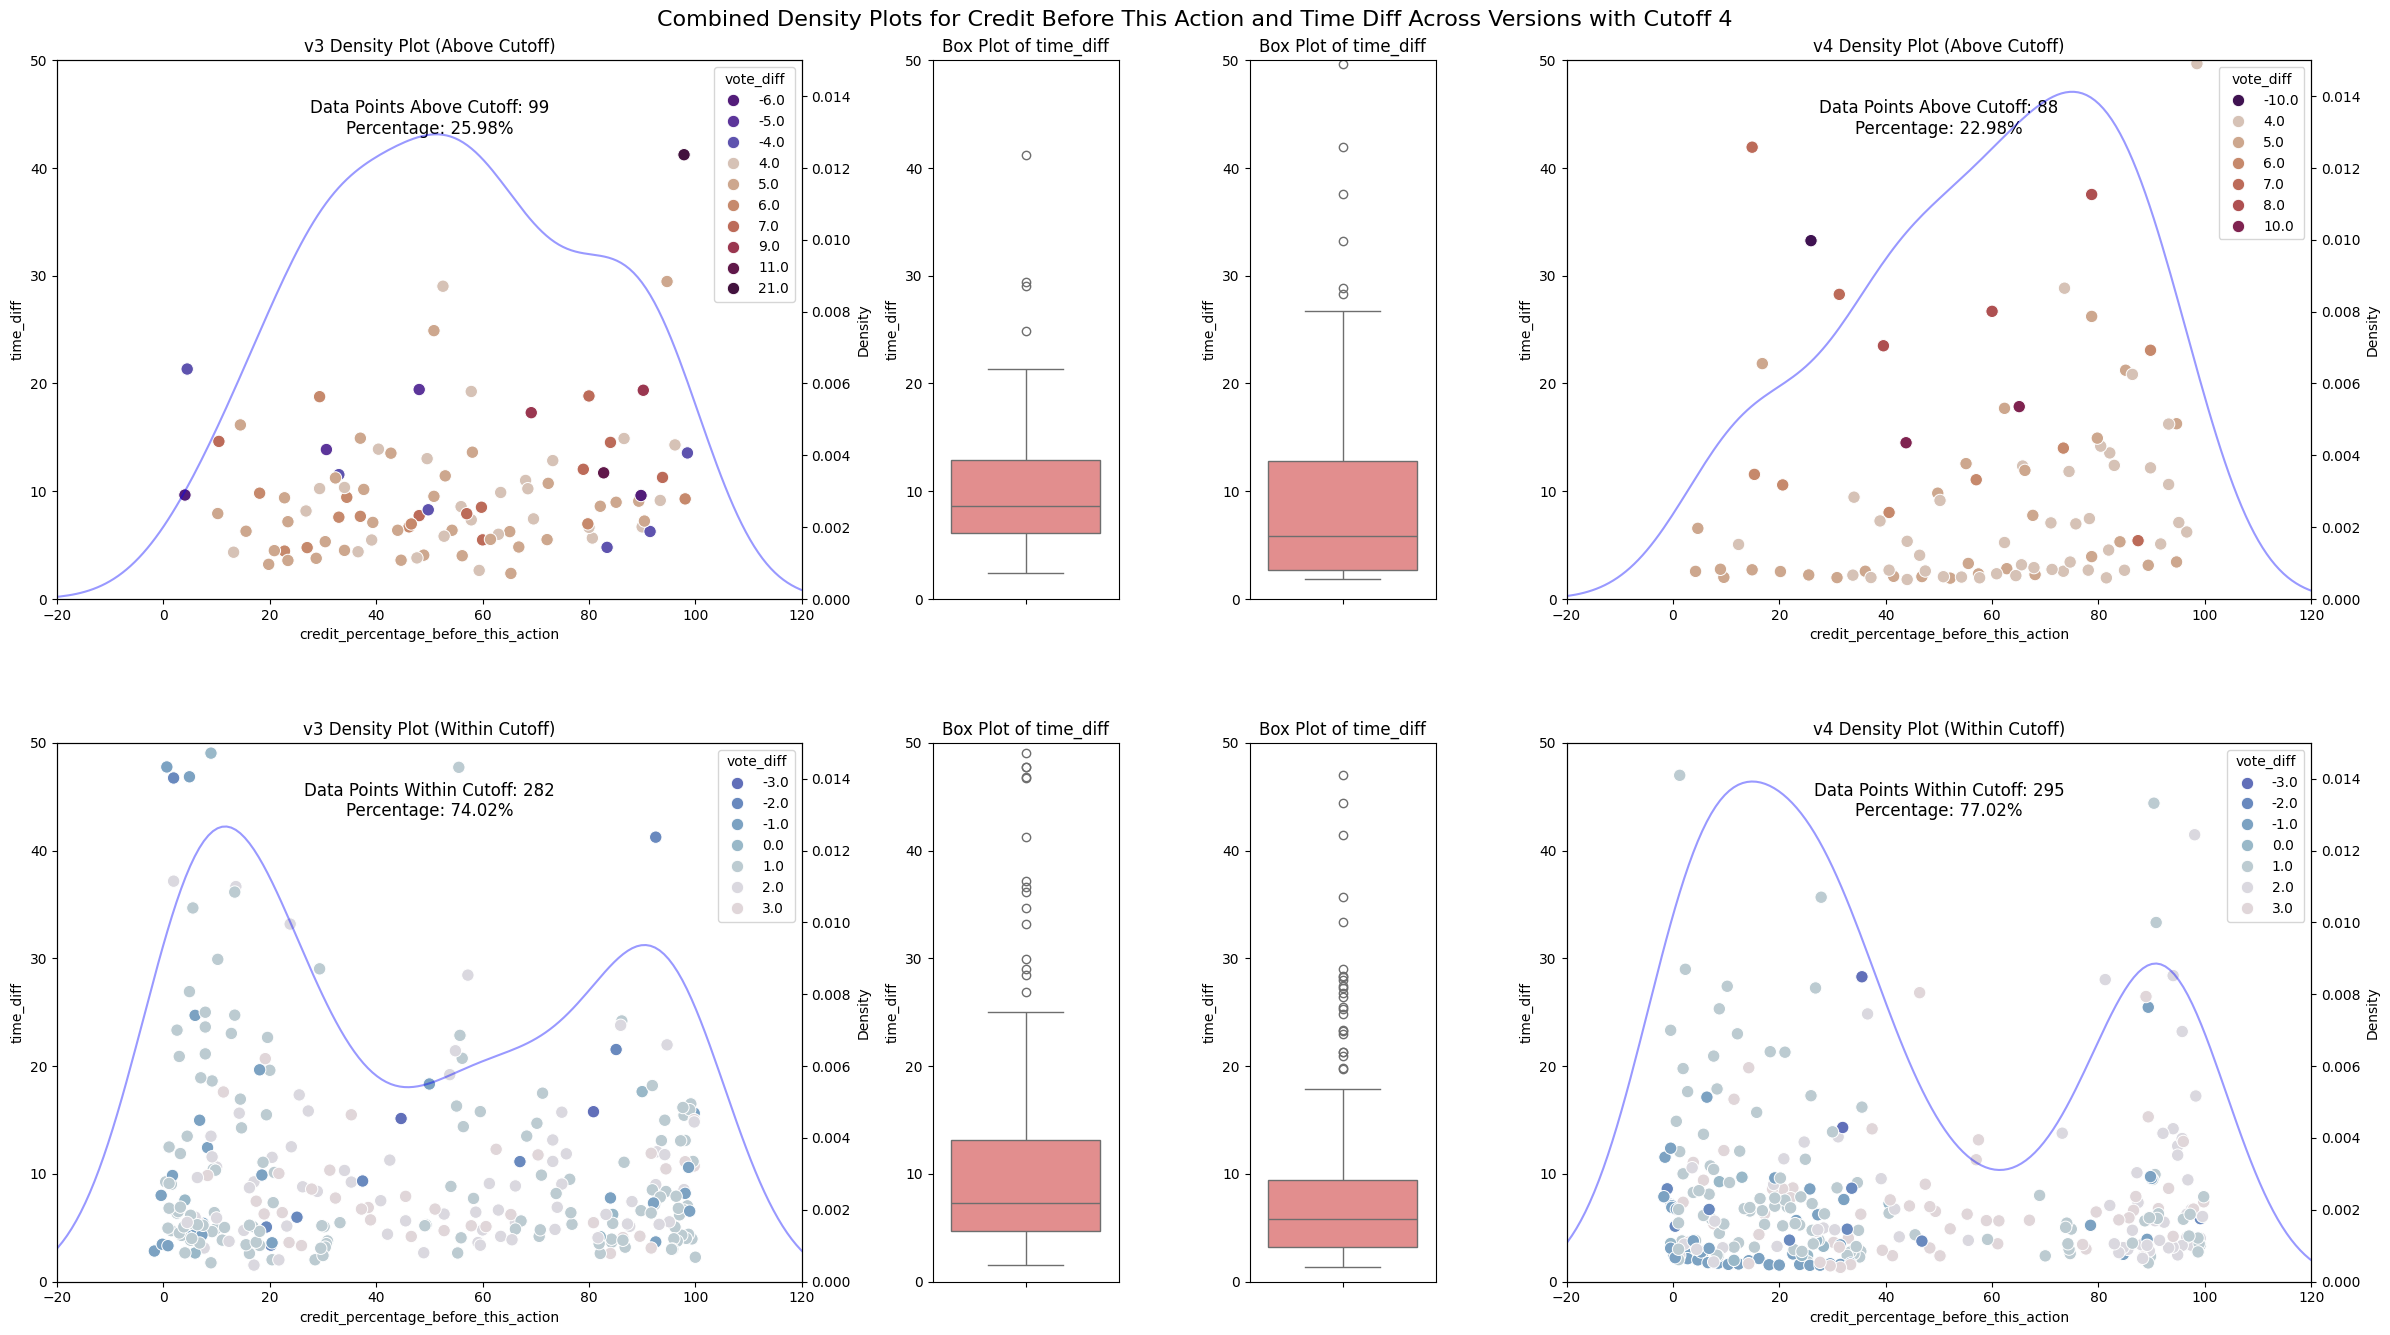
\includegraphics[width=\textwidth]{content/image/results/temp_cut4.png}
    \caption{Breakdown of voting actions (needs to update chart text)}
    \label{fig:voting_v3_v4}
\end{figure}

Thus, we further separated the behaviors where participants made bigger changes or smaller changes to the option, specifically for the long version. In Figure~\ref{fig:voting_v3_v4} , we define an adjustment of four or more votes as a large adjustment which we plotted in the first row of the Figure. Adjustments of three or fewer votes are considered small adjustments.

First, we are able to surface the bimodal action distribution in both plots, with a even stronger signal for long interactive interface participants. Second, the plot demonstrated a clear cluster of voting actions in the bottom left corner of the interactive interface for small vote adjustments. In other words, participants made much smaller but more rapid adjustments when their budgets were running low. Second, larger adjustments are made when the participants have more options comparing the two plots on the first row. We interpret this behavior as participants in the interactive interface have constructed a clearer image of option preferences and, hence, have the ability to take larger strides in allotting their budget and deciding the number of votes at the beginning of the survey. Toward the end, participants using the interactive interface are then making fine-tuned adjustments to ensure that their preferences are reflected in their submissions.

% add qualitative support
\paragraph{Iterative Support from Interactive Interface}
Among all the interviews, when discussing about their experience of the interface, five particpants pointed out the importance of flexibility on the interface and how they took an incremental and iterative approach to navigating their attitude expression. All these participants are using the interactive interface. While this does not mean the study participant using the text interface did not use an iterative approach, but this highlighted the interactive interface encouraged the participants to make iterative and incremental updates. As one participant pointed out:

\begin{displayquote}
I like the fact that it remembers everything that you know. If if you make a mistake, that you don't lose all the work that you've already done. so I think that's very important is that it's an iterative process.

\noindent \hfill -- S019, long interactive interface.
\end{displayquote}

\subsection{Interface Comments}
Finally, we present the qualitative responses related to the interface design and their experience working with QS across all experiment groups.

\paragraph{Organization is required and beneficial}
Many participants (N=7) who responded to QS using the interactive interface expressed the helpfulness of the organization phase proactively when asked what they liked about the interface in general. In fact, half of the participants (N=5) in the long interactive interface group expressed such an opinion. Multiple participants (N=4, 3 from long interactive interface group) felt that the upfront introduction of all the topics allowed them to process and think about the full picture, thereby digesting all the information more comprehensively. 

\begin{displayquote}
I would say that (the interface) definitely (supported me), by being able to have a preliminary categorization of all the topics. First, it introduced me to all the topics, so that I can think about them like I can just kind of leave it there in my head space to think about and process \bracketellipsis So being able to digest all the information prior to actually allocating the budget or completing the quadratic survey.

\noindent \hfill -- S009, long interactive interface.
\end{displayquote}

% \begin{displayquote}
% \bracketellipsis having some sort of categories helped in establishing these 3 categories is like the first tip, and then, like I said, I have other categories myself~\bracketellipsis classifying things into categories~\ldots\ make me~\ldots\ I don't know \ldots\ It was just easier for me. 

% \noindent \hfill -- S021, long interactive interface.
% \end{displayquote}

Participants (N=4, 2 from long interactive interface group) mentioned that organization support them to allot the intensity of votes by helping them focus and prioritize options through ranking options. This excercise allows them to follow a clear decision making process that avoids confusion.

\begin{displayquote}
If I had to choose a number like that in the beginning. That would have been really bad, but positive, neutral, negative. That was good enough.

\noindent \hfill -- S016, long interactive interface.
\end{displayquote}

\begin{displayquote}
I think \ldots\ ranking at the beginning one's impression towards these issues helps to like determine how many votes should be put towards them. 

\noindent \hfill -- S002, short interactive interface.
\end{displayquote}

Last, one participants highlighted the one-at-a-time approach during the organization phase allowed thoughtful reflection to think about their attitude toward that option.

\begin{displayquote}
Like, at the moment (during organization), when it gives you, like, rank it if it's positive or neutral or negative~\bracketellipsis it gives you time to just focus on that single thing and rank it based on how you feel at that moment.
    
    \noindent \hfill -- S013, short interactive interface.
\end{displayquote}

We see a call for organizational features proactively when asking participants using the text-based interface what features they wanted from the interface. Almost half of the participants (N=4) using the long text interface expressed some form or another that can help reduce the decision space when responding to the QS.

\begin{displayquote}
    If anything, I think I would like to be able to like, click and drag the categories themselves so I could maybe reorder them to like my priorities.
        
        \noindent \hfill -- S025, long interactive interface.
\end{displayquote}

\begin{displayquote}
    Because with this many (options), especially when I'm thinking \ldots\ Ok, where was (the option) \ldots\ Where was (the option) you know? Oh, that's right. Maybe I could give another up another upvote to the, you know whatever~\bracketellipsis
        
        \noindent \hfill -- S028, long interactive interface.
\end{displayquote}

\paragraph{Direct Manipulation Enhances Reflective Decision-Making}
As the proximity of position are mostly determined by the categorization in the first phase of the interactive interface. Several participants mentioned how they used direct Manipulation in the software as a process for reflective thinking upon their decision making process. One participant mentioned:

\begin{displayquote}
So I tried to make a ranking~\bracketellipsis and by creating this ranking, by dragging the related issues~\ldots\~i don’t know~\ldots\~that helped me organize my ideas.
    
\noindent \hfill -- S021, long interactive interface.
\end{displayquote}

\begin{displayquote}
I think the system was actually really helpful because I could just drag them.~\bracketellipsis Because when I was unsure, because if I couldn't drag them then I couldn't compare 2 options very well like side to side, because because this is pretty long list~\ldots\ so if I couldn't drag it, then I would have a harder time organizing my thoughts, whereas  with the dragging feature I can really compare them, I can drag this one up here, and then compare it to the top one versus like not being able to track it at all
    
\noindent \hfill -- S039, long interactive interface.
\end{displayquote}


But more importantly, it acts as a process for reflective verification and iterative decision making. These can include post reflection after expressing the intesnsitve of preferences, or a preperation to decide on number of votes for the next option.


\begin{displayquote}
So I would give the votes, and then I would drag and drop.~\bracketellipsis So I guess to see what my ranking look like. And see if I could give more money or not.
    
\noindent \hfill -- S021, long interactive interface.
\end{displayquote}

\begin{displayquote}
\bracketellipsis this is something that's really important to me \ldots\ So I had the flexibility to move it to positive. So just having the kind of like shift in perception. ~\bracketellipsis especially because when I was doing categorize categorization in the first step, ~\bracketellipsis what I thought about it in the moment. ~\bracketellipsis In the second step there was a shift in my perception of the issue just reflecting. So being able to change. That was really nice as well. 

\noindent \hfill -- S009, long interactive interface.
\end{displayquote}

Conversely, in the text interface, one participant proactively mentioned a request to add click and drag functionalities to the interface. The participants described such function to group by topic categorization and also priority placement through direct manipulation. 

\begin{displayquote}
If anything, I think I would like to be able to like, click and drag the categories themselves so I could maybe reorder them to like my priorities. And so I could maybe make that like a descending or ascending like list of like importance.~\bracketellipsis if I could pull that up to the top, say myself like click and drag it up there, I think then I would stack the things I think it would affect under it. So like, I would put then, like youth, pro-education programs and adult education and early childhood programs and kinda stack those altogether.~\bracketellipsis I would hope that money would trickle down and also increase all the rest of those things. So I would put less upvotes in there because I would hope to dribble out effect would kick in.~\bracketellipsis I would kind of make myself categories and subcategories out of this list. If I could organize it.

\noindent \hfill -- S025, long text interface.
\end{displayquote}

\paragraph{Automatic calculation as a critical component}
More than one-third of participants (N=14) from all four experiment condition highlighted the importance of automated calculation from two perspectives:~\textit{deriving cost} and ~\textit{Keeping track of spent}. Two participant highlighted the importance of automated calculation regarding the cost for each vote.

\begin{displayquote}
I really like having the costs of all the votes displayed. When you select the dropdown menu and ranked in order.

\noindent \hfill -- S002, short interactive interface.
\end{displayquote}

$12$ participants highlighted the summarization box and the automated summation of the current credit spent allowed them to focus on managing their next voting decision and express their preferences.

\begin{displayquote}
I thought I have~\bracketellipsis (to) do all the numbers or calculation myself as a part of checking my ability of doing mathematics. But I guess you have taken care of that really well, so I could really really see that how much credit has left, and~\bracketellipsis how well I should allocate~\bracketellipsis I said that credit summary to be very specific. The credit summary section was really wonderful in doing all the calculation on that end.

\noindent \hfill -- S005, long text interface.
\end{displayquote}

\begin{displayquote}
I like that I don't have to make the calculation of the dollars that it does it automatically. So if I had to do it myself it would be more tedious. And so I think that that effort and frustration and mental demand would be much higher. So I appreciate that that calculation occurs automatically and very easily. 

\noindent \hfill -- S017, short interactive interface.
\end{displayquote}



% Ti-Chung Cheng: So what elements of the software interface do you dislike, or like the most, if any, when expressing your preferences on responding to societal issues?
% S009: Hmm! What I like the most actually, probably the sorting function. I think that it really helped me organize my thoughts really, clearly, in terms of what I would dislike the most. really, not that much. I would say. yeah, also, like how we could categorize it, like even within the voting stage rather than just at the categorization stage. 

% Ti-Chung Cheng: Can you tell me a little bit more about the screen? How did the vertical screen help you?
% S037: I think because it helps the layout of, because it's like a long 3 bar. So it's easier for you to to drag and drop, and you can actually sort it, judging by the votes. But I do not do that. But I think this layout is could be helpful in that aspect.

